\documentclass[10pt,twocolumn,letterpaper]{article}

\usepackage{cvpr}
\usepackage{times}
\usepackage{epsfig}
\usepackage{graphicx}
\usepackage{amsmath}
\usepackage{amssymb}

% Include other packages here, before hyperref.

% If you comment hyperref and then uncomment it, you should delete
% egpaper.aux before re-running latex.  (Or just hit 'q' on the first latex
% run, let it finish, and you should be clear).
\usepackage[breaklinks=true,bookmarks=false]{hyperref}

\cvprfinalcopy % *** Uncomment this line for the final submission

\def\cvprPaperID{****} % *** Enter the CVPR Paper ID here
\def\httilde{\mbox{\tt\raisebox{-.5ex}{\symbol{126}}}}

% Pages are numbered in submission mode, and unnumbered in camera-ready
%\ifcvprfinal\pagestyle{empty}\fi
\setcounter{page}{1}
\begin{document}

%%%%%%%%% TITLE
\title{Using a Generic Camera as a Scanner}

\author{
Colin Schmidt, Nicholas Sunjaya, Yi Hong To\\
UC Berkeley\\
{\tt\small \{colins, nicholas.sunjaya, craigyihongto\}@berkeley.edu}
}

\maketitle
%\thispagestyle{empty}

\begin{abstract}
   The ABSTRACT is to be in fully-justified italicized text, at the top
   of the left-hand column, below the author and affiliation
   information. Use the word ``Abstract'' as the title, in 12-point
   Times, boldface type, centered relative to the column, initially
   capitalized. The abstract is to be in 10-point, single-spaced type.
   Leave two blank lines after the Abstract, then begin the main text.
   Look at previous CVPR abstracts to get a feel for style and length.
\end{abstract}

\section{Introduction}
\label{sec:intro}

Scanning documents has been a common practice for a long time.
Even before the advent of digital scanners faxes were a popular of sending documents to others.
But as smartphones have become more ubiquitous and fully featured they have begun to absorb many features of other electronics.

In this paper we present an algorithm for turning a simple smartphone camera, or any other camera, into a scanner.
The properties of a scanner we will replicate are: the page scanned fills the image, it is orientated with the top of the page at the top of the image, and that the ratio of the image is the same as that of the paper.

We first describe our motivation for developing this tool in section~\ref{sec:motivate}.
Next, we introduce our multi-step algorithm with illustrations in section~\ref{sec:algorithm}.
Following this is a description of our experimental methodology and the results of applying the algorithm to a set of images in section~\ref{sec:results}.
Then, we discuss which images are problematic for our algorithm and potential solutions in section~\ref{sec:discuss}.
Finally, in section~\ref{sec:conclude} we conclude with an exploration of future work and highlight out successes.

\section{Motivation}
\label{sec:motivate}

Here we will explain why people need our project.

\section{Algorithm}
\label{sec:algorithm}

Our algorithm is a multi-step process that identifies the bounding box of the item and then use homography transform to produce the final image.
We will now walk through the algorithm with a sample image seen in figure~\ref{fig:normal}.

\begin{figure}[t]
\begin{center}
   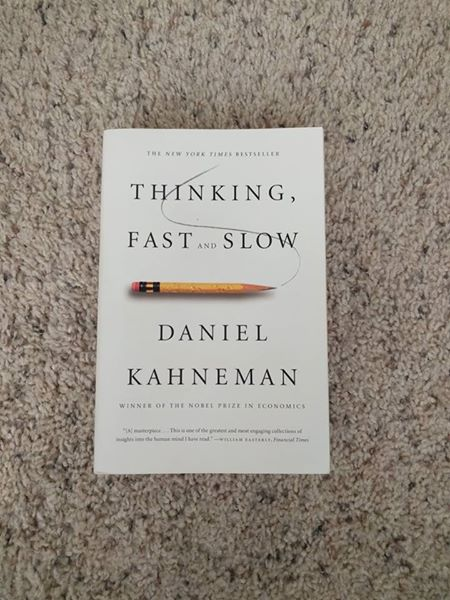
\includegraphics[width=0.8\linewidth]{figures/normal.jpg}
\end{center}
\caption{What the image looks like before any modification.}
\label{fig:normal}
\end{figure}

The first step of the algorithm is to identify edges in the image.
We converted the images to gray scale.
Then we smooth the image with a gaussian filter to help remove some background noise.
Then we use a canny edge detector to give us the binary image of edges.
Because of the non-maximal supression the canny edge detector, it gives us the best chance of getting fine lines.
Fine lines enable the next steps in our algorithm to be more precise.
The output of the edge dection can be seen in figure~\ref{fig:edge}.

\begin{figure}[t]
\begin{center}
   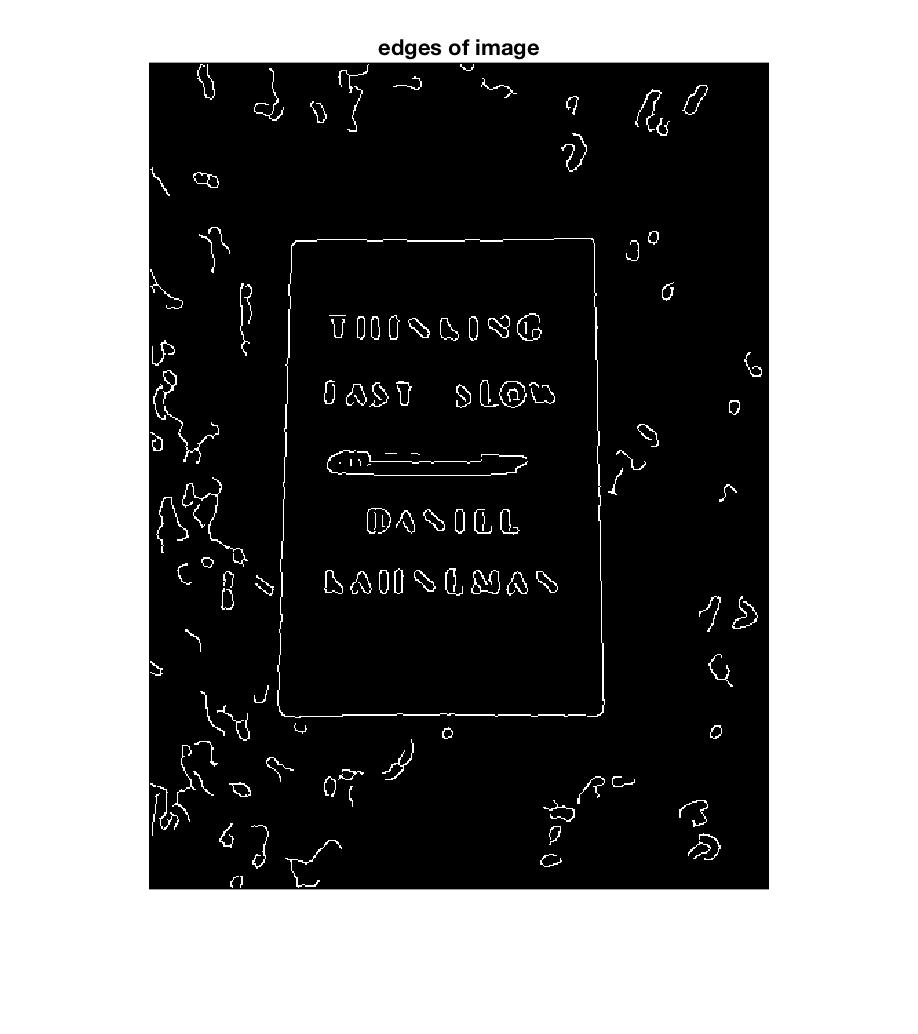
\includegraphics[width=0.8\linewidth]{figures/edgeDetection.jpg}
\end{center}
\caption{After edge-detection.}
\label{fig:edge}
\end{figure}

Once we have the binary image of edges we need to detect which edges correspond to straight lines.
To accomplish this we use the Hough transform~\cite{hough}.
Hough transform indentifies lines by keeping track of the pixels in terms of their slope.
If a bunch of pixel belongs to a line, they should have the similar slope with respect to a starting point.
The Hough transform algorithm keep track and score the collection of pixels.
We set this transformation such that gives us up to 10 line candidates.
These prospective lines can be seen in figure~\ref{fig:lines}

\begin{figure}[t]
\begin{center}
   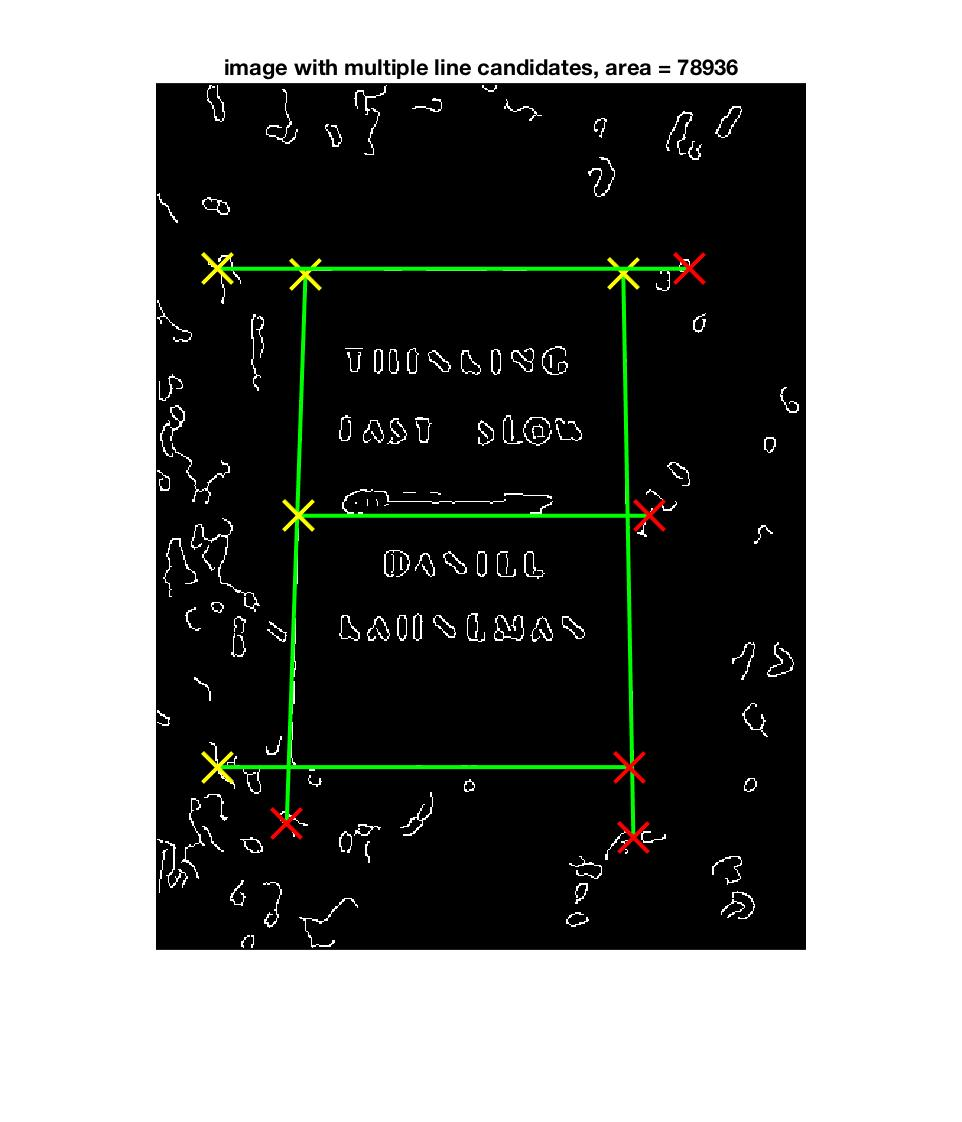
\includegraphics[width=0.8\linewidth]{figures/step2.jpg}
\end{center}
\caption{The second step}
\label{fig:lines}
\end{figure}

Next we use a random sampling method inspired by RANSAC to pick the lines that best represent the item.
In this step we use some assumptions about the images to develop a heuristic for which lines should be best.
Hough transform returns the coordinates of the endpoints of the lines.
From there, we can compute the vector that parametrizes the line.
To determine the corner, which is the intersection of a horizontal and vertical line, we perform cross product on the vectors of the lines.
We assume that the largest quadrilateral in the image is the item, such that maximizing the area of our polygon will be the correct bounding box for our item.
We also assume that it will be approximately rectangular, such that lines forming near right angles are preferred over acute or obtuse angles.
Using this criteria we then randomly sample four lines from the set keeping track of which best meets our heuristic.
At the end of this process we have four lines we believe to lie on the bounding box of the item.
With these lines we then find their intersections and mark these as the corners of the item.
The result of this step can be seen in figure~\ref{fig:box}.


\begin{figure}[t]
\begin{center}
   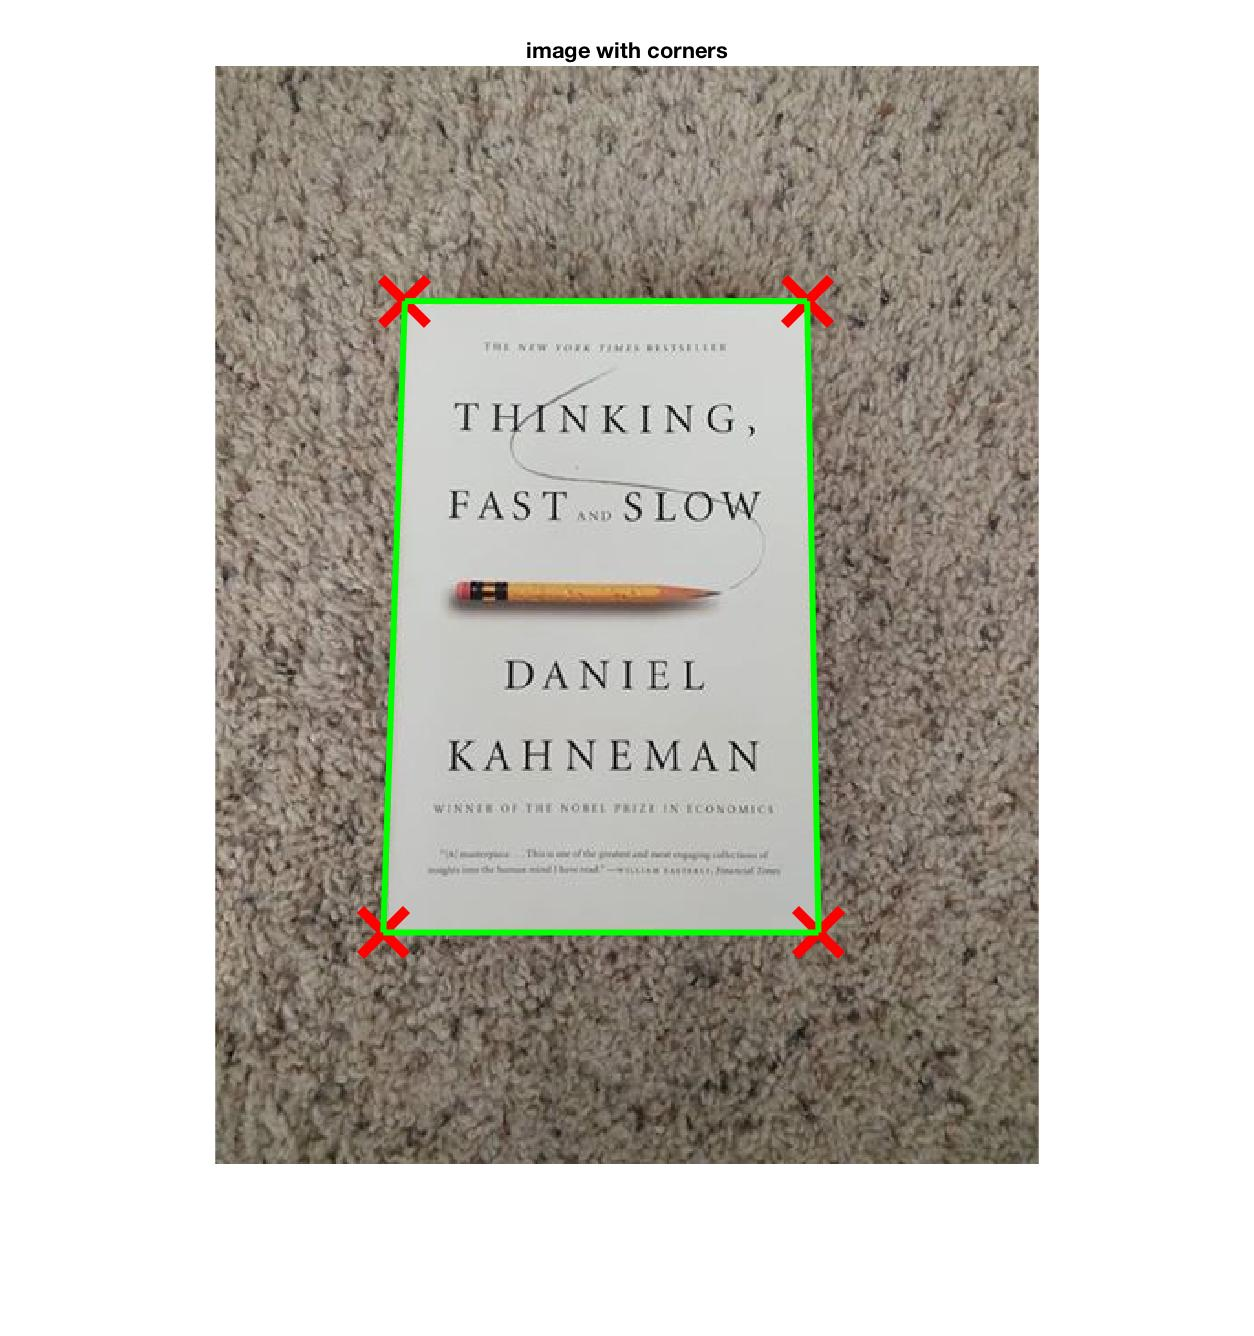
\includegraphics[width=0.8\linewidth]{figures/step3.jpg}
\end{center}
\caption{The third step}
\label{fig:box}
\end{figure}

Finally we use this set of corners as the input to a homography transformation.
Once we have computed the transform we then transform all pixels in the bounding box to get the final image as seen in figure~\ref{fig:final}.


\begin{figure}[t]
\begin{center}
   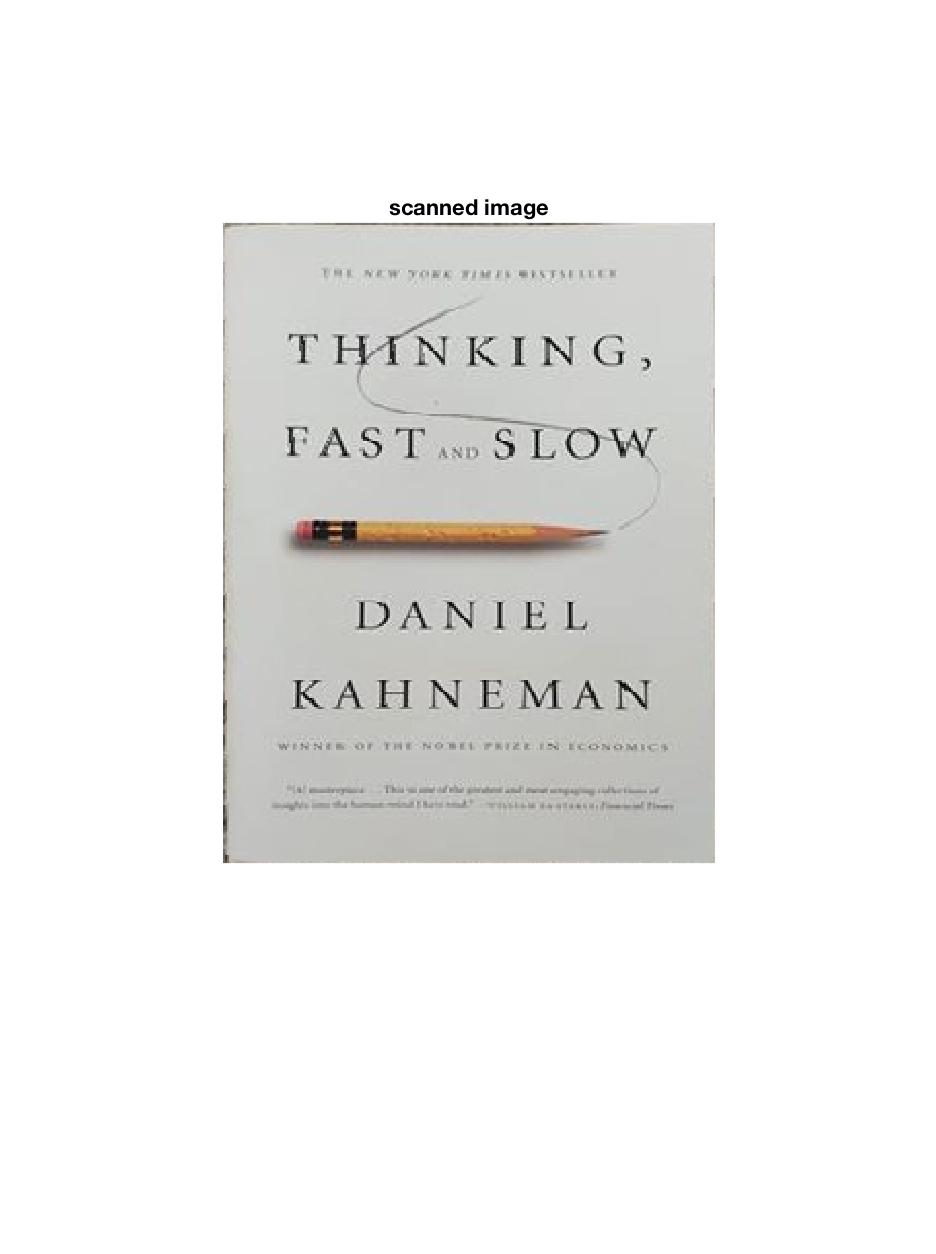
\includegraphics[width=0.8\linewidth]{figures/step4.jpg}
\end{center}
\caption{The fourth step}
\label{fig:final}
\end{figure}

\section{Results}
This section will summarize our results maybe in a table like~\ref{tab:example}.
And maybe some largerer figures like~\ref{fig:short}.

\begin{figure*}
\begin{center}
\fbox{\rule{0pt}{2in} \rule{.9\linewidth}{0pt}}
\end{center}
   \caption{Example of a short caption, which should be centered.}
\label{fig:short}
\end{figure*}

\begin{table}
\begin{center}
\begin{tabular}{|l|c|}
\hline
Method & Frobnability \\
\hline\hline
Theirs & Frumpy \\
Yours & Frobbly \\
Ours & Makes one's heart Frob\\
\hline
\end{tabular}
\end{center}
\caption{Results.   Ours is better.}
\label{tab:example}
\end{table}

\section{Discussion}
\label{sec:discuss}

Even though we have a decent success rate for most images there are some particular failure modes that are worht talking about.

\subsection{Fewer Edges}
The first such scenario is where the edges of the item are simply difficult to detect.
In figure~\ref{fig:missedEdge} the Canny edge detector is unable to find the right edge of the paper.
This kind of error could be adressed potentially with more pre-processing of the image.
There is a tradeoff with this type of error and some of the future errors which are results of having too many edges.
If we have the edge detector identify more edges it becomes difficult to pick the right set.

\begin{figure}[t]
\begin{center}
   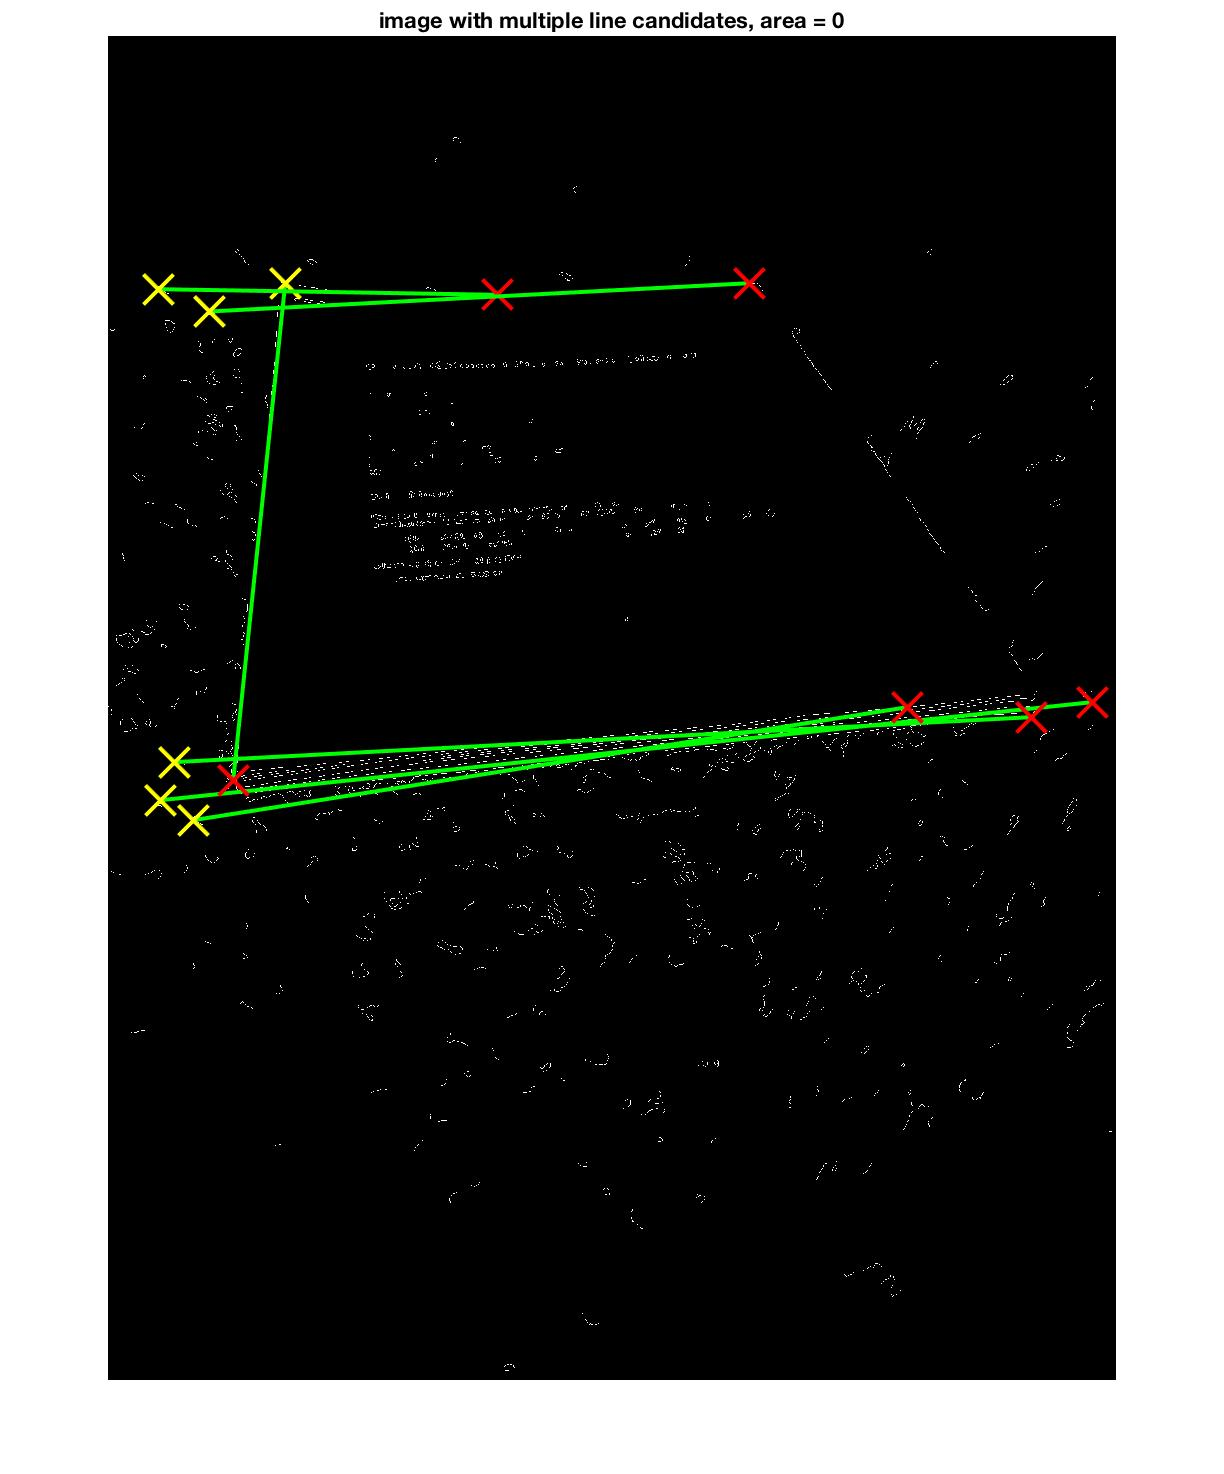
\includegraphics[width=0.8\linewidth]{figures/missedEdge.jpg}
\end{center}
\caption{An image which has an undetectable edge.}
\label{fig:missedEdge}
\end{figure}


\subsection{Extra Edges}
The remaining types of errors fall into a different category where we have detected edges that do not correspond to the actual edges of the book cover.

The first failure mode we see is where the book has significant depth that also has a sharp edge with the background as in figure~\ref{fig:depthError}.
This causes the largest bounding box to include an additional edge of the book that is not the true edge of the cover.
One heuristic to possibly detect the difference between the cover and the side of the book would be to expect that side of the book will often be a consistent cover, e.g. white.
Then if we find that we have two quadrilaterals to pick from and one of them is essentially the other but with a large monochrome segement attached we can guess that this is the side of the book.


\begin{figure}[t]
\begin{center}
   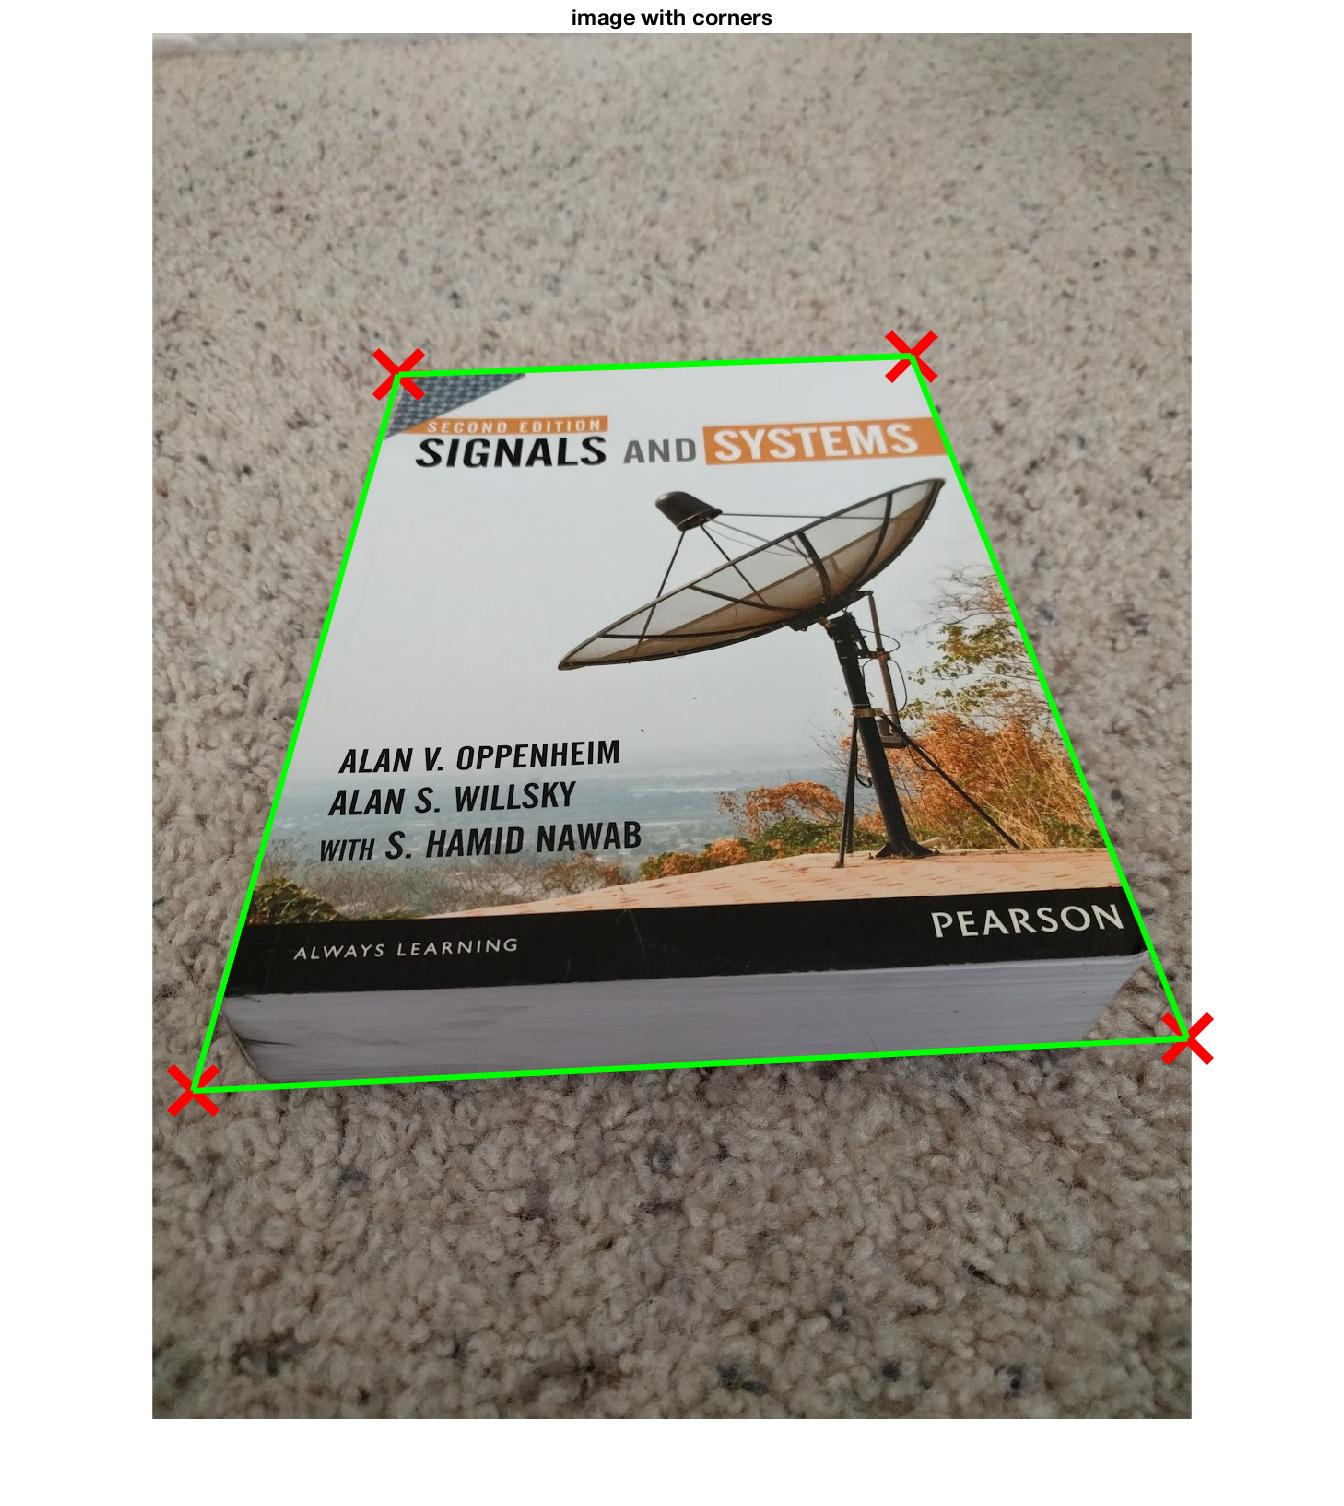
\includegraphics[width=0.8\linewidth]{figures/depthError.jpg}
\end{center}
\caption{A book which is deep and thus has a larger rectangle than the correct one.}
\label{fig:depthError}
\end{figure}

A similar failure mode appears in figure~\ref{fig:shadowError}.
However in this failure rather than the side of the book it is the shadow of the book that creates the larger false rectangle.
This failure seems similar enought to the previous mode that the same heuristic may work well again.
If the shadow is solid enough to be detected as an additional line then it is probably monochrome just like the side of the book.
In our example image this turns out to be true and so we hypothesize that using the same monochrome attachement heurstic from before could correct this image.

\begin{figure}[t]
\begin{center}
   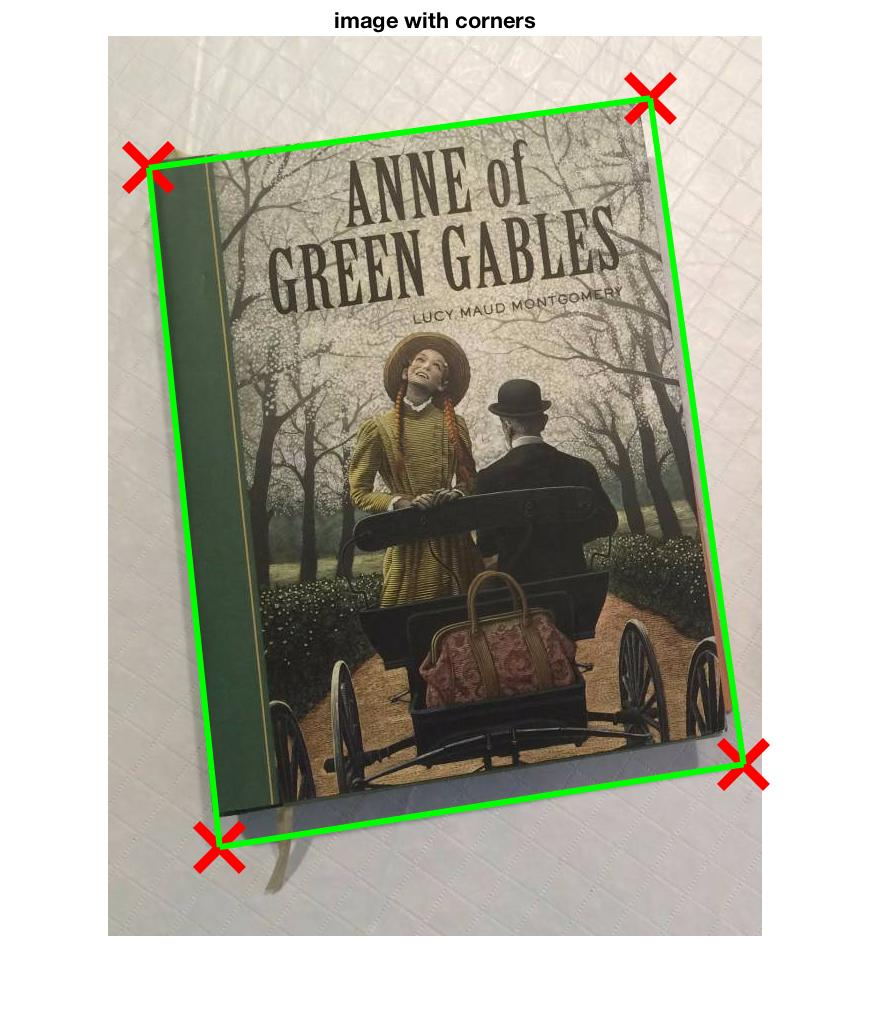
\includegraphics[width=0.8\linewidth]{figures/shadowError.jpg}
\end{center}
\caption{A book which has a well defined shadow and thus a larger rectangle than the correct one.}
\label{fig:shadowError}
\end{figure}

Finally the last failure mode we discuss is that of extra lines on the cover of the book or page.
These are actual lines that should be detected by any sensible edge detector but cause problems with our bounding box selection as seen in figure~\ref{fig:extraEdges}.
This is certainly our most difficult to handle failure mode, and has no clear solution of mitigation technique.

\begin{figure}[t]
\begin{center}
   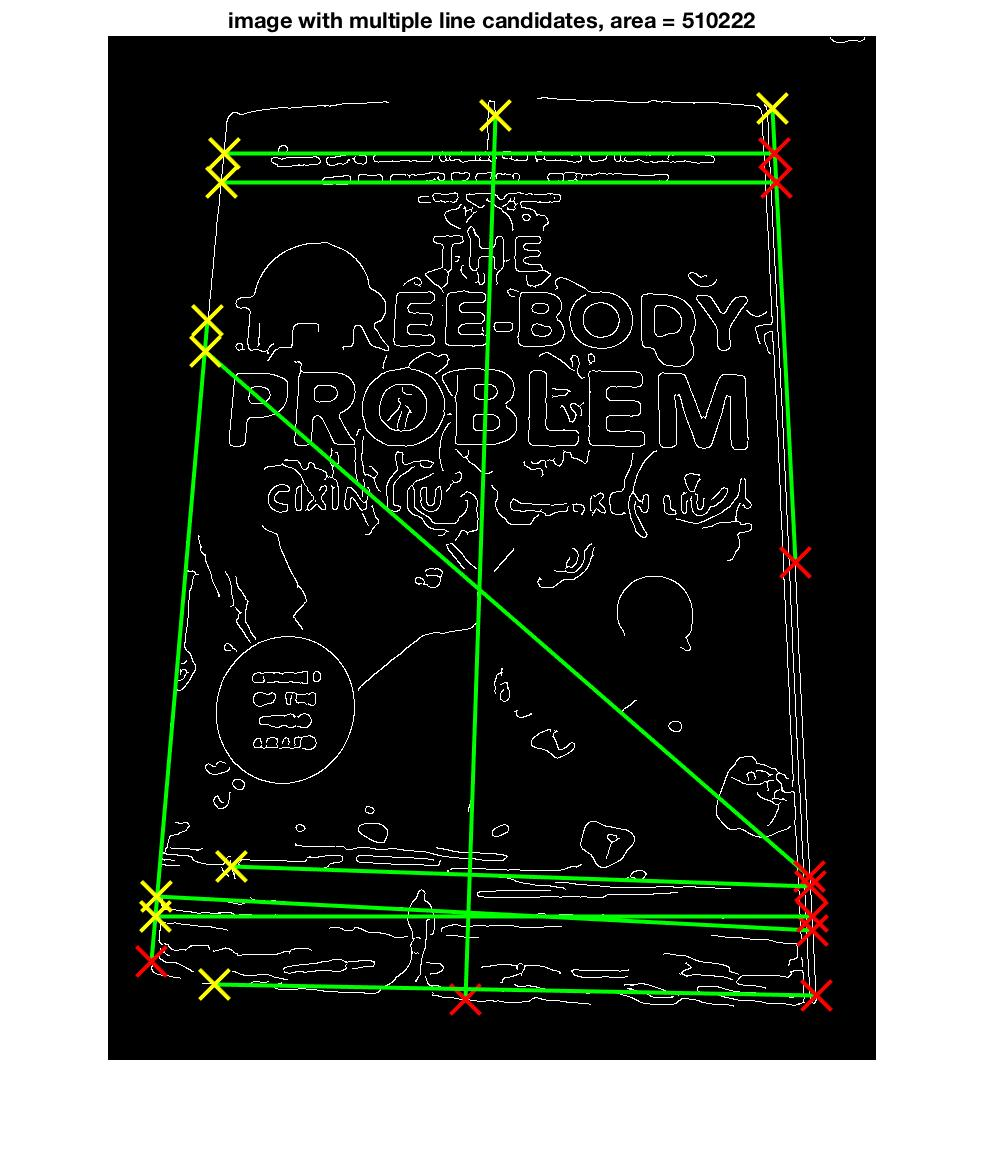
\includegraphics[width=0.8\linewidth]{figures/extraEdges.jpg}
\end{center}
\caption{A book which has a lot of extra edges on the cover making it hard to find the right set of four.}
\label{fig:extraEdges}
\end{figure}

\section{Conclusion}
\label{sec:conclude}

Overall our algorithm is able to acheieve a 71\% accuracy rating on a diverse set of book and papers with interesting and varied backgrounds.
There are several particular failure modes that could be addressed with additional some heuristics.
We believe the algorithm remains useful as a cammer to scanner conversion despite these hiccups.



{\small
\bibliographystyle{ieee}
\bibliography{egbib}
}

\end{document}
